\section{Results}
\label{sec:results}
\subsection{User Experience}
TODO: Annie
    -Terms of Service
    -Setup to home router
    -Using the internet
    -Experience
    -Cookie experience (Fourthparty)

\subsection{Teardown}
TODO: Annie
    -Parts in the box
    -Possible attacks via USB/SD Card

\begin{figure}[htb]
\begin{center}
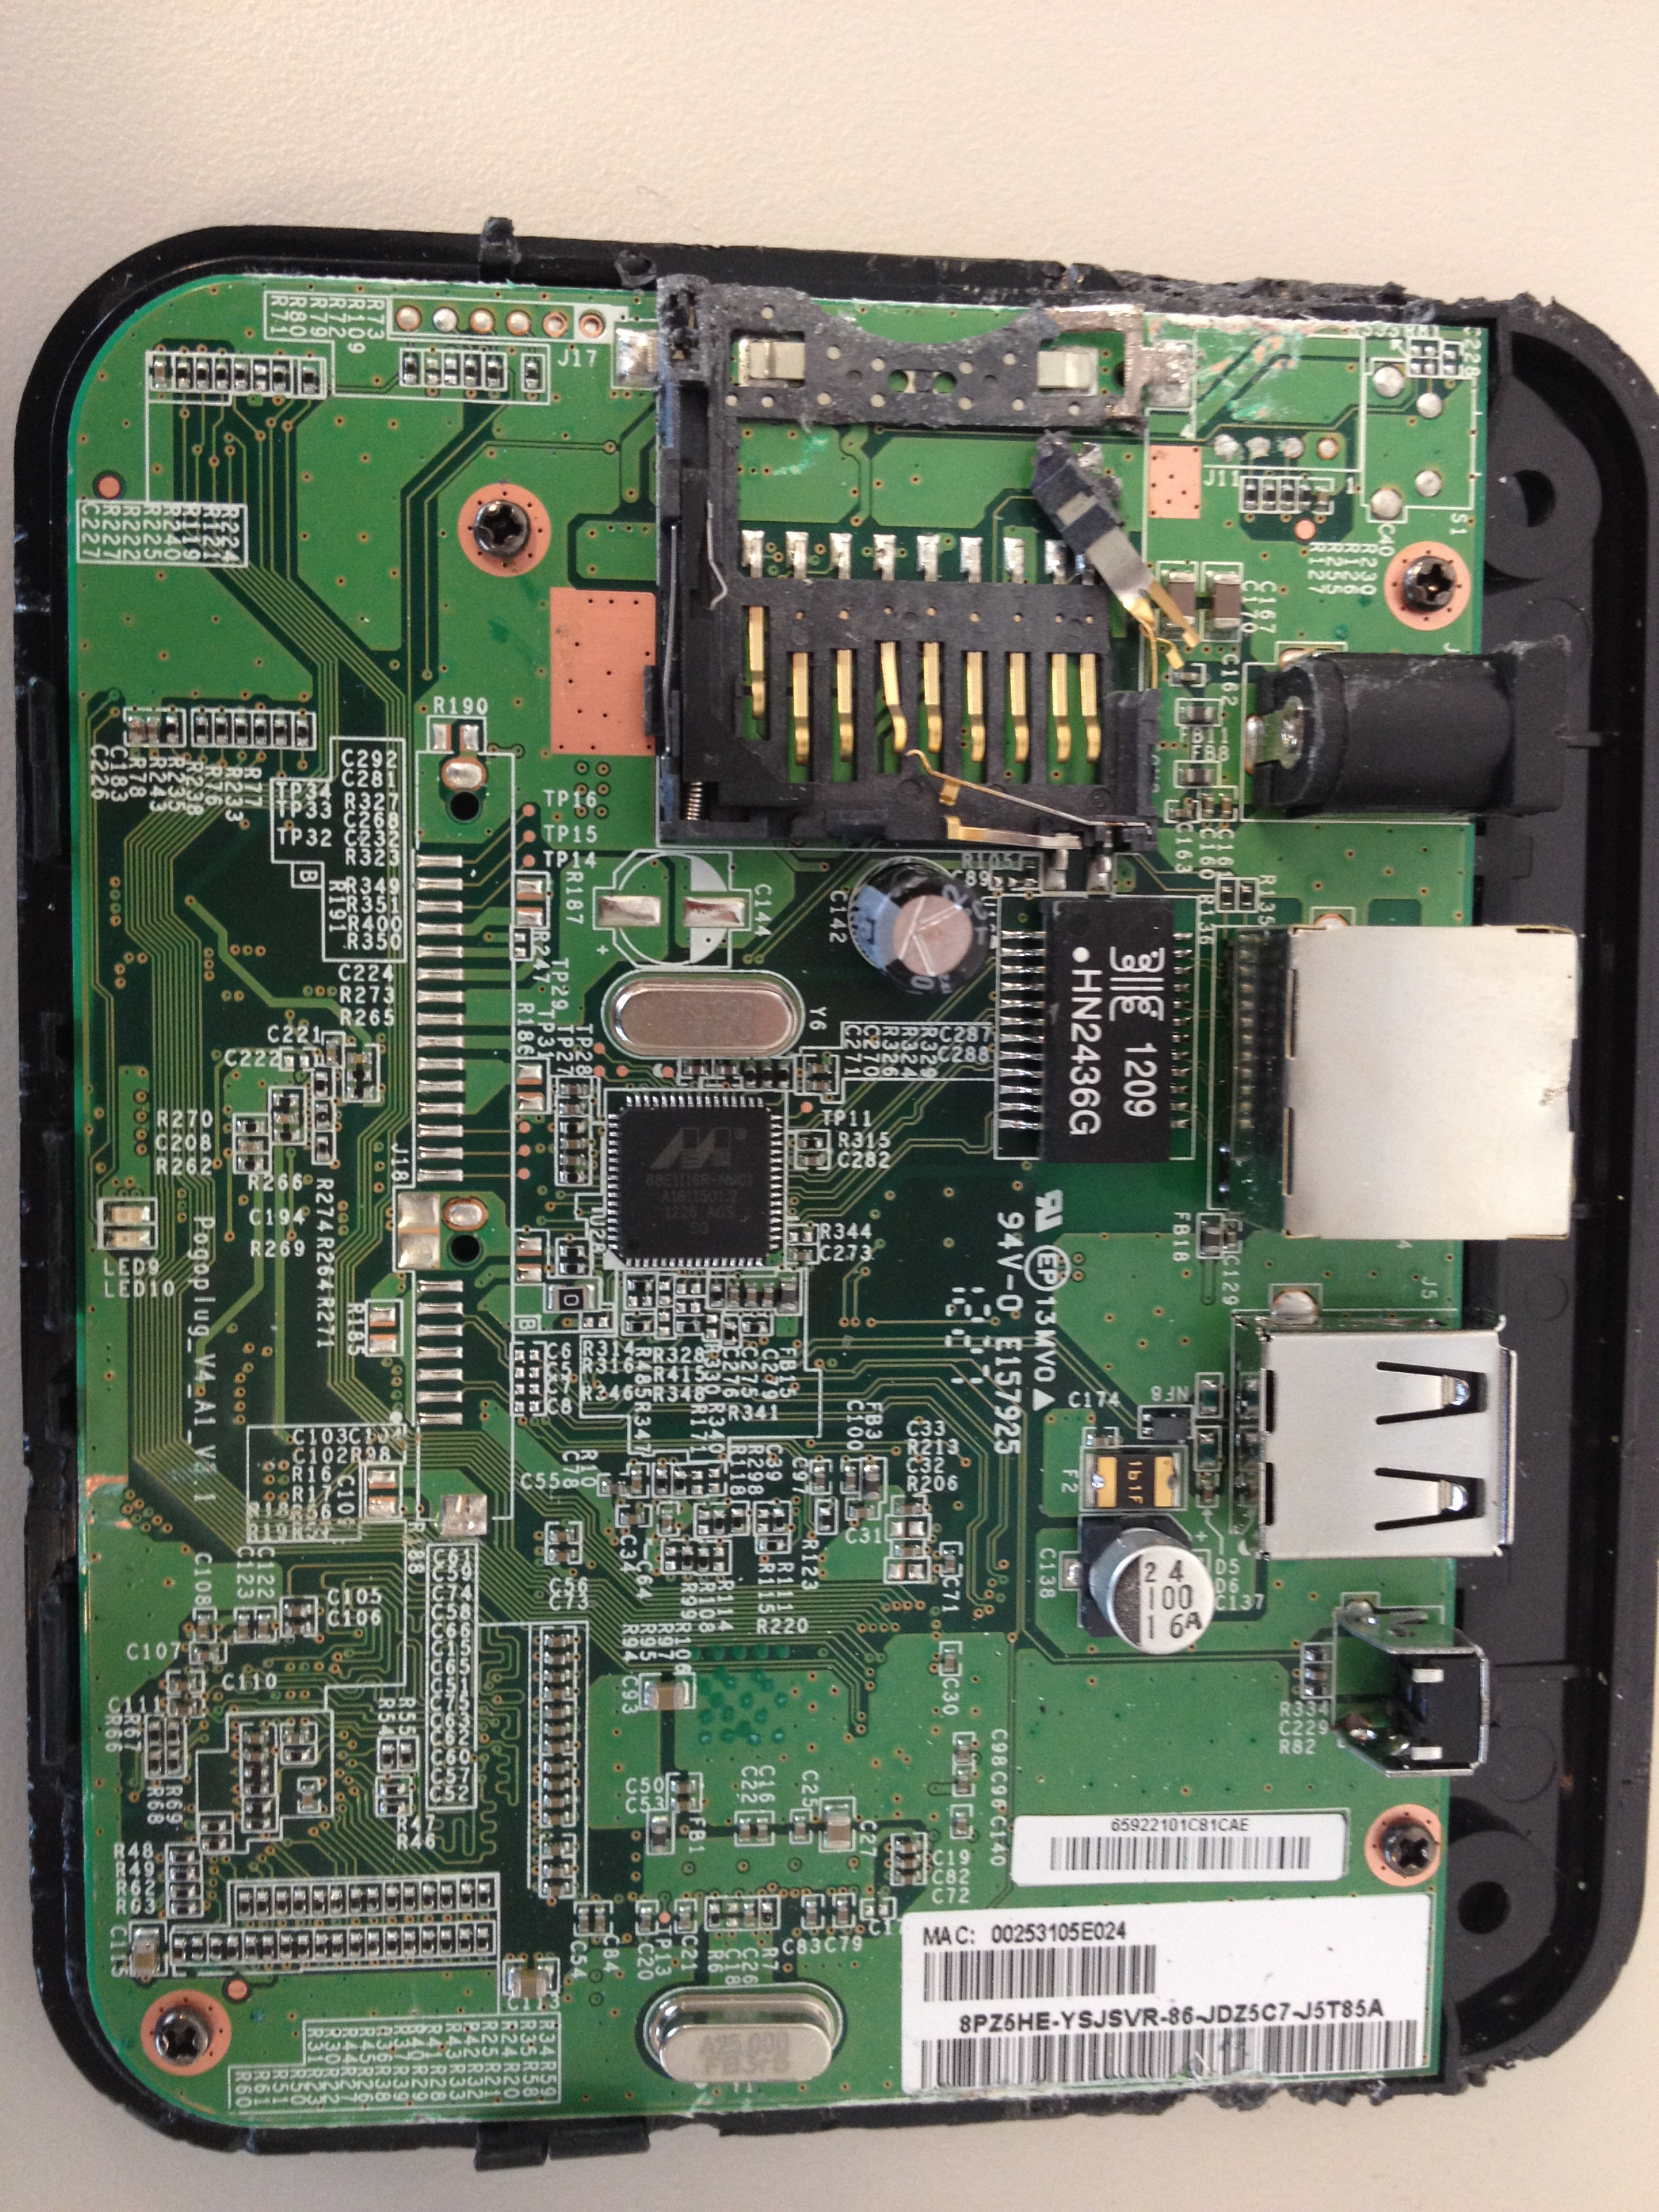
\includegraphics[width=\linewidth]{safeplug_top}
\caption{This is a figure.}
\end{center}
\end{figure}

\begin{figure}[htb]
\begin{center}
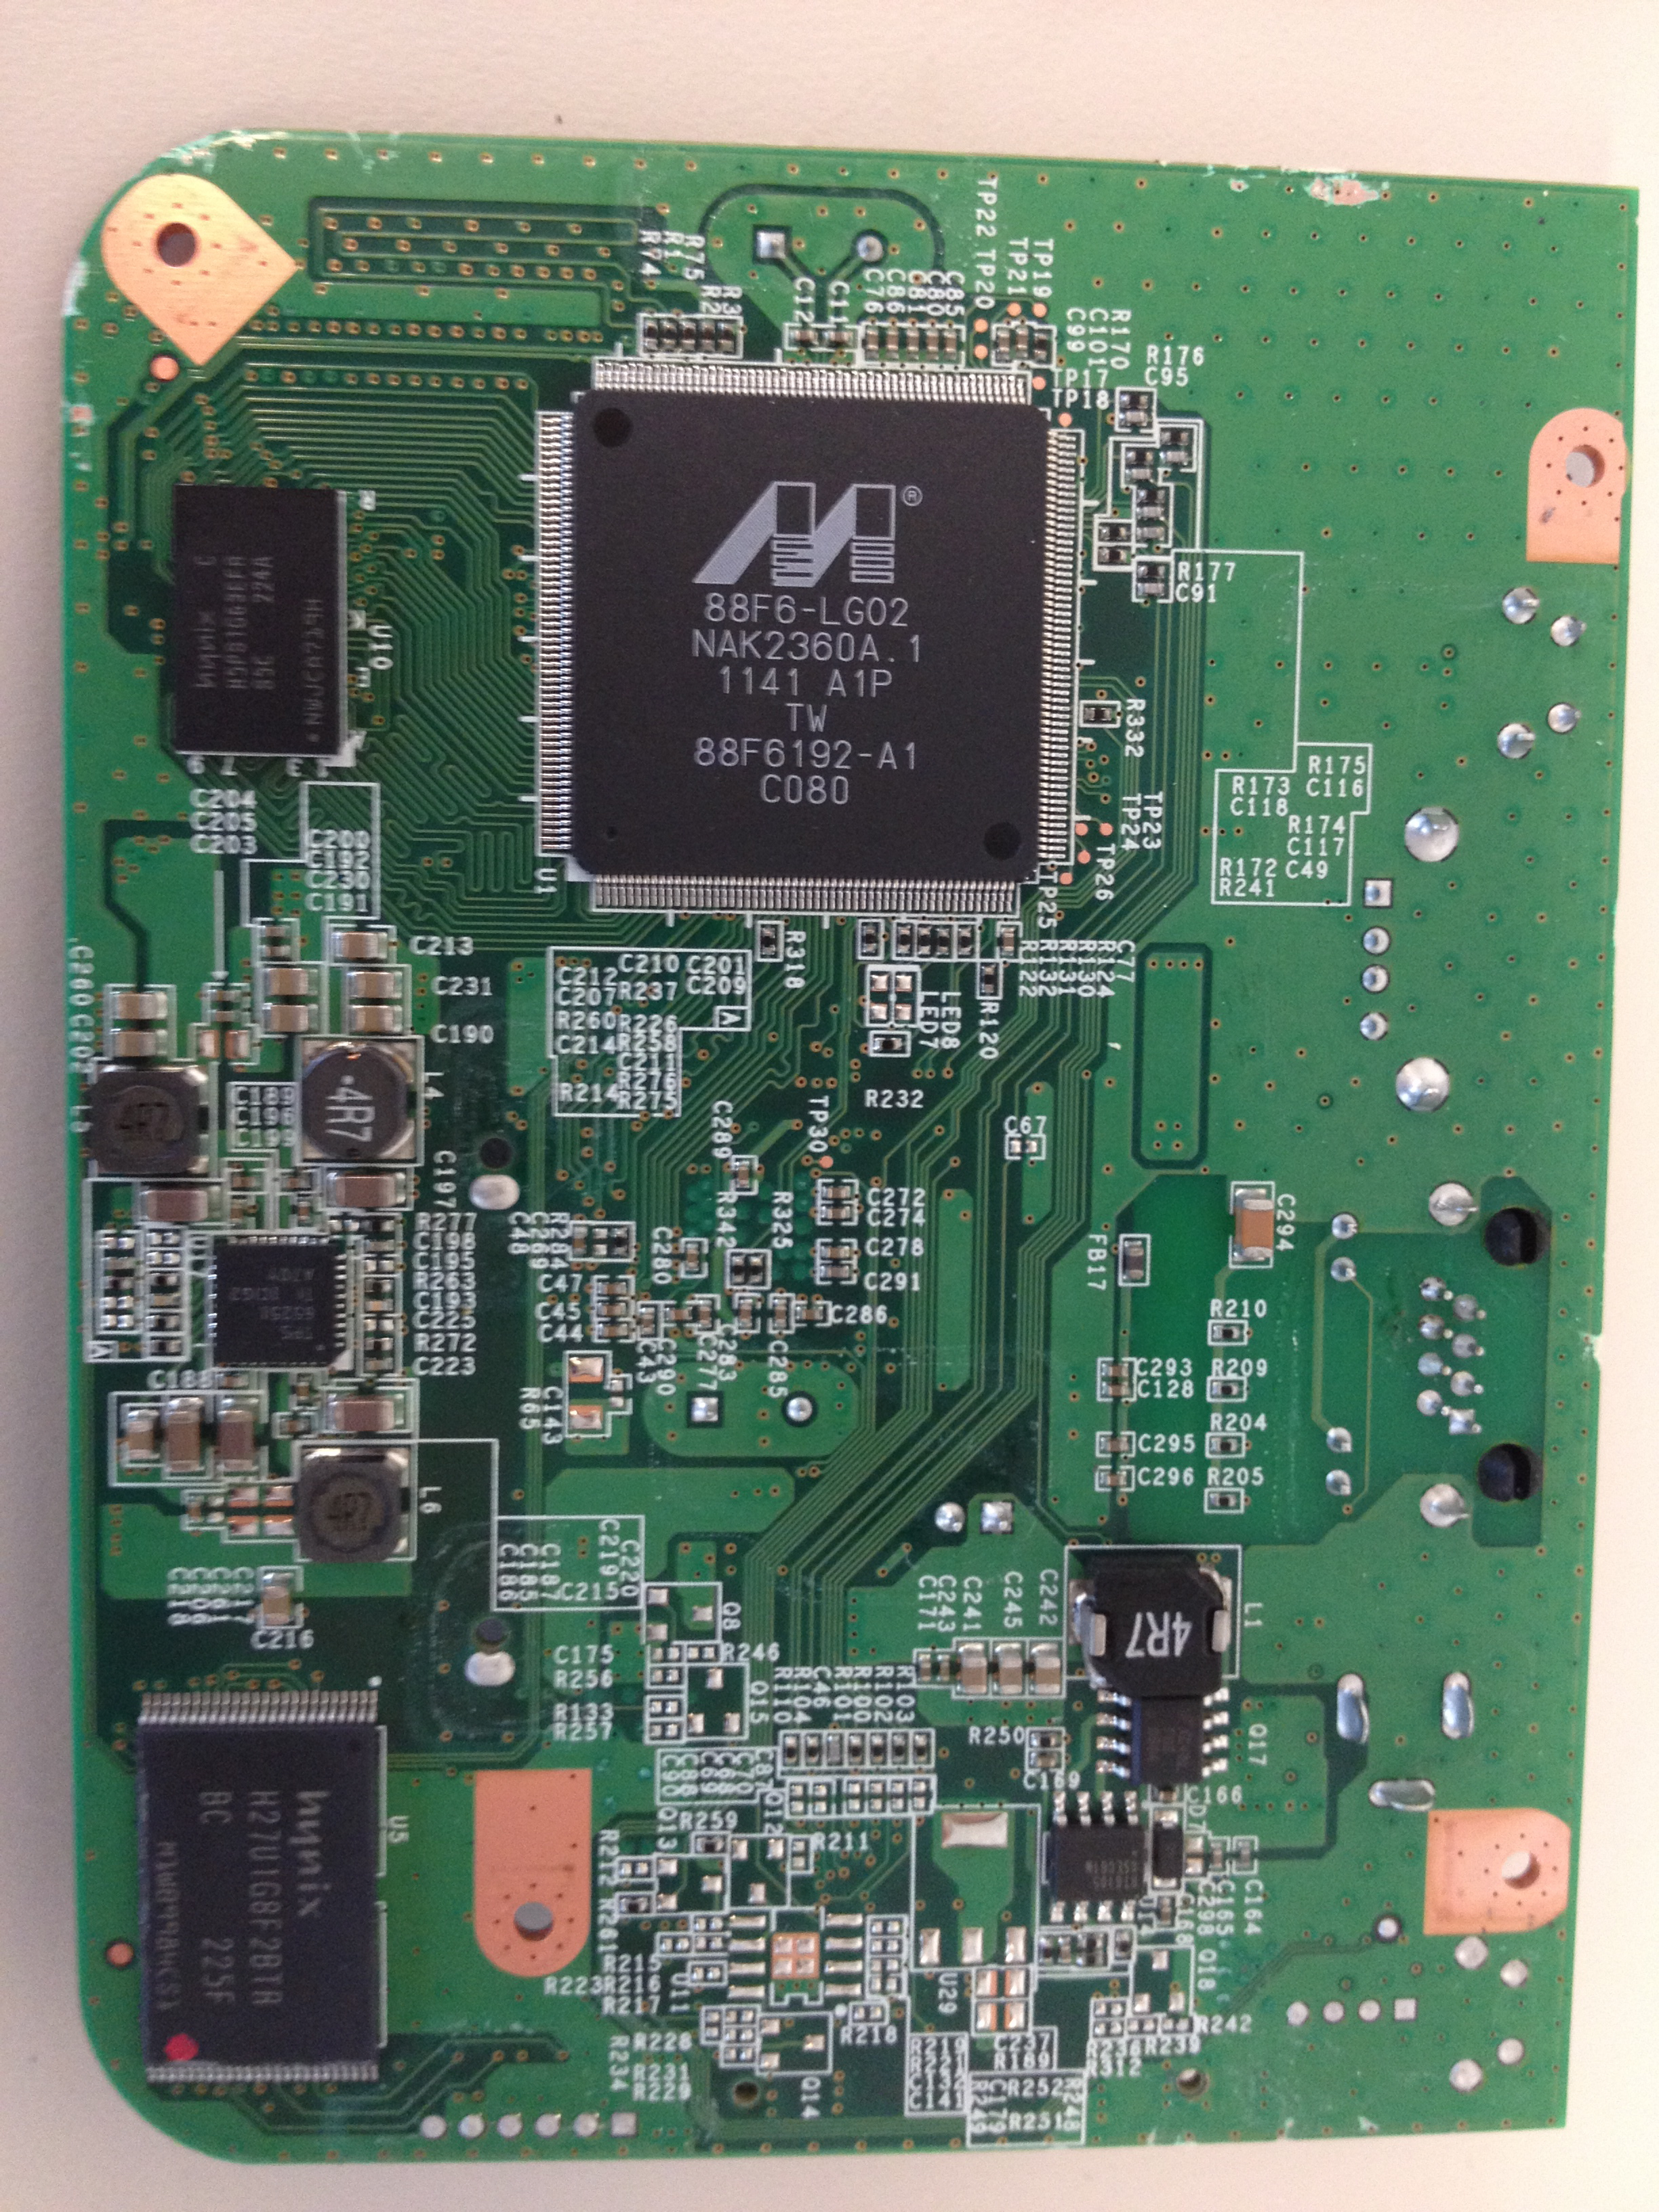
\includegraphics[width=\linewidth]{safeplug_bottom}
\caption{This is a figure.}
\end{center}
\end{figure}

\subsection{Traffic Analysis}
TODO: Anna
    -What's the udpate?
    -Phone home frequency
    -Does it do anything else?
    -How does the ad-blocking work?

\subsection{Gaining Access through SSH}
TODO: Anna
    -How we got access
    \subsubsection{Accessing the Device}
    -What's the software
    \subsubsection{Software on the Safeplug}
Tor, Privoxy, and Lighttpd.  Lighttpd is an open-source webserver, which is serving the settings page on the device - the project's description mentions ``security, speed, compliance, and flexibility [... while being] designed and optimized for high perfomance environments'' \cite{lighttpd}.  Privoxy is a ``non-caching web proxy with advanced filtering capabilities for enhancing privacy, modifying webpage data and HTTP headers, controlling access, and removnig ads and other obnoxious Internet junk'' and it specifically advertises its ``flexible configuration'' \cite{privoxy}.
    -What/where are the settings
    -RPC server
        -Attacks from anyone on local network
        -Attack from a website?
